\documentclass{standalone}
\usepackage{tikz}
\usetikzlibrary{patterns, positioning}


\begin{document}
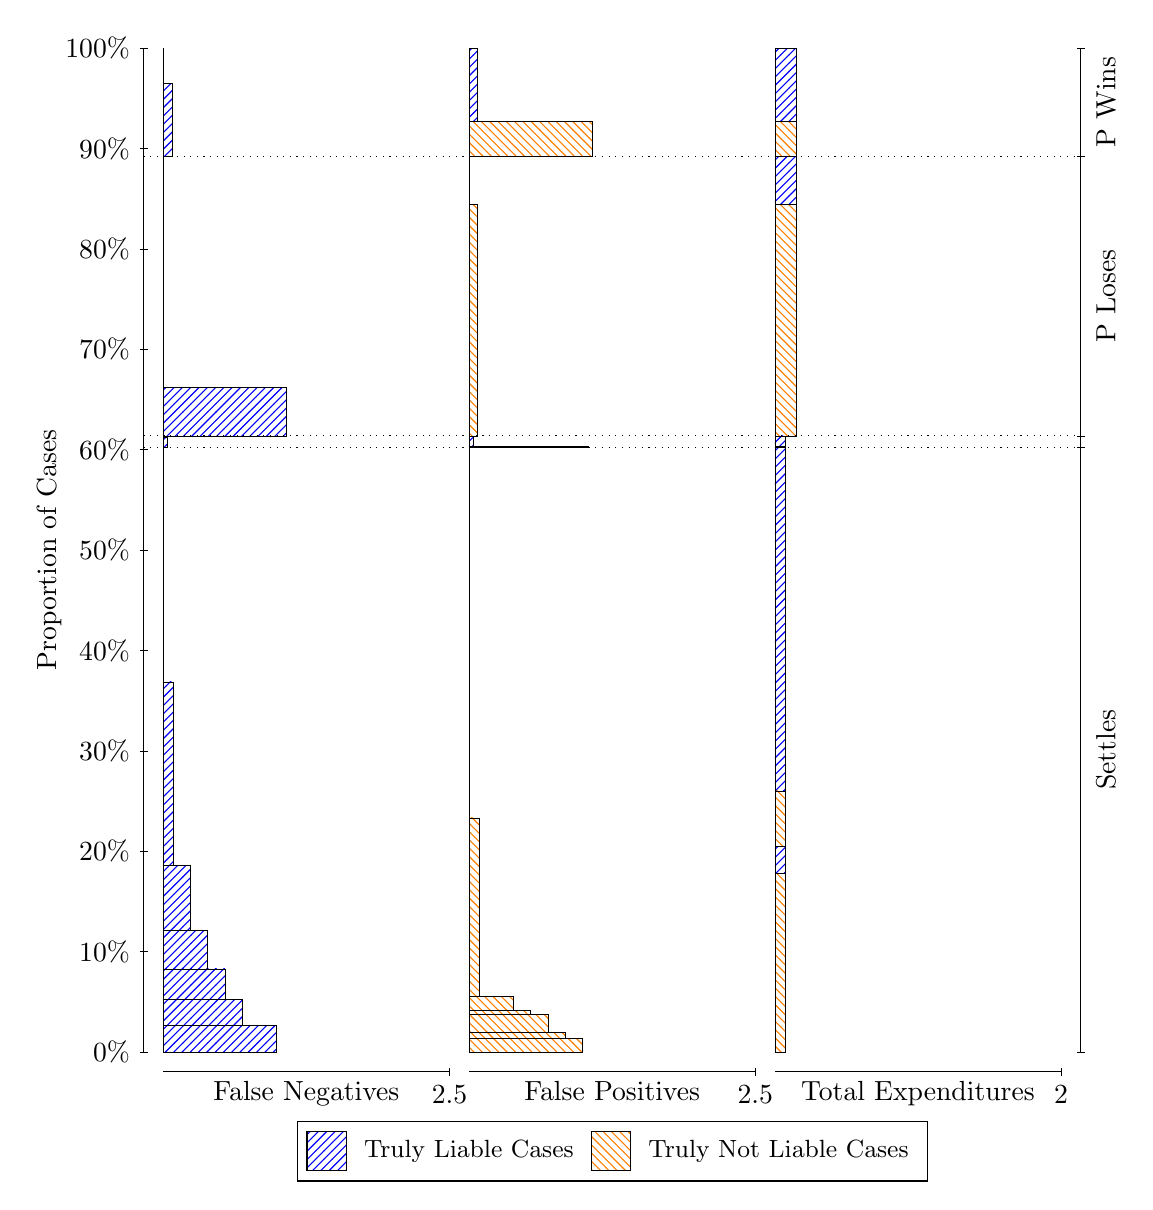
\begin{tikzpicture}
\draw[black, very thin] (1.5,1.75) -- (1.5,14.5);
\node[rotate=90, text=black, anchor=center] at (0.3, 8.125) {Proportion of Cases};
\draw[black, very thin] (1.45,1.75) -- (1.55,1.75);
\node[text=black, anchor=east] at (1.45, 1.75) {0\%};
\draw[black, very thin] (1.45,3.025) -- (1.55,3.025);
\node[text=black, anchor=east] at (1.45, 3.025) {10\%};
\draw[black, very thin] (1.45,4.3) -- (1.55,4.3);
\node[text=black, anchor=east] at (1.45, 4.3) {20\%};
\draw[black, very thin] (1.45,5.575) -- (1.55,5.575);
\node[text=black, anchor=east] at (1.45, 5.575) {30\%};
\draw[black, very thin] (1.45,6.85) -- (1.55,6.85);
\node[text=black, anchor=east] at (1.45, 6.85) {40\%};
\draw[black, very thin] (1.45,8.125) -- (1.55,8.125);
\node[text=black, anchor=east] at (1.45, 8.125) {50\%};
\draw[black, very thin] (1.45,9.4) -- (1.55,9.4);
\node[text=black, anchor=east] at (1.45, 9.4) {60\%};
\draw[black, very thin] (1.45,10.675) -- (1.55,10.675);
\node[text=black, anchor=east] at (1.45, 10.675) {70\%};
\draw[black, very thin] (1.45,11.95) -- (1.55,11.95);
\node[text=black, anchor=east] at (1.45, 11.95) {80\%};
\draw[black, very thin] (1.45,13.225) -- (1.55,13.225);
\node[text=black, anchor=east] at (1.45, 13.225) {90\%};
\draw[black, very thin] (1.45,14.5) -- (1.55,14.5);
\node[text=black, anchor=east] at (1.45, 14.5) {100\%};

\draw[black, very thin] (13.4,1.75) -- (13.4,14.5);
\draw[black, very thin] (13.35,1.75) -- (13.45,1.75);
\node[anchor=west] at (13.35, 1.75) {};
\draw[black, very thin] (13.35,9.4247) -- (13.45,9.4247);
\node[anchor=west] at (13.35, 9.4247) {};
\draw[black, very thin] (13.35,9.5753) -- (13.45,9.5753);
\node[anchor=west] at (13.35, 9.5753) {};
\draw[black, very thin] (13.35,13.125) -- (13.45,13.125);
\node[anchor=west] at (13.35, 13.125) {};
\draw[black, very thin] (13.35,14.5) -- (13.45,14.5);
\node[anchor=west] at (13.35, 14.5) {};

\draw[black, very thin, pattern color=blue, pattern=north east lines] (1.75,1.75) rectangle (3.1852,2.0908);
\draw[black, very thin, pattern color=blue, pattern=north east lines] (1.75,2.0908) rectangle (2.7492,2.417);
\draw[black, very thin, pattern color=blue, pattern=north east lines] (1.75,2.417) rectangle (2.5312,2.8058);
\draw[black, very thin, pattern color=blue, pattern=north east lines] (1.75,2.8058) rectangle (2.3132,3.2989);
\draw[black, very thin, pattern color=blue, pattern=north east lines] (1.75,3.2989) rectangle (2.0952,4.1174);
\draw[black, very thin, pattern color=blue, pattern=north east lines] (1.75,4.1174) rectangle (1.8772,6.4505);
\draw[black, very thin, pattern color=orange, pattern=north west lines] (1.75,6.4505) rectangle (1.75,9.4247);
\draw[black, very thin, pattern color=blue, pattern=north east lines] (1.75,9.4247) rectangle (1.8045,9.5572);
\draw[black, very thin, pattern color=orange, pattern=north west lines] (1.75,9.5572) rectangle (1.75,9.5753);
\draw[black, very thin, pattern color=blue, pattern=north east lines] (1.75,9.5753) rectangle (3.3123,10.188);
\draw[black, very thin, pattern color=orange, pattern=north west lines] (1.75,10.188) rectangle (1.75,13.125);
\draw[black, very thin, pattern color=blue, pattern=north east lines] (1.75,13.125) rectangle (1.859,14.054);
\draw[black, very thin, pattern color=orange, pattern=north west lines] (1.75,14.054) rectangle (1.75,14.5);
\draw[black, very thin, pattern color=orange, pattern=north west lines] (5.6333,1.75) rectangle (7.0685,1.9254);
\draw[black, very thin, pattern color=orange, pattern=north west lines] (5.6333,1.9254) rectangle (6.8505,2.0006);
\draw[black, very thin, pattern color=orange, pattern=north west lines] (5.6333,2.0006) rectangle (6.6325,2.2321);
\draw[black, very thin, pattern color=orange, pattern=north west lines] (5.6333,2.2321) rectangle (6.4145,2.2745);
\draw[black, very thin, pattern color=orange, pattern=north west lines] (5.6333,2.2745) rectangle (6.1965,2.457);
\draw[black, very thin, pattern color=orange, pattern=north west lines] (5.6333,2.457) rectangle (5.7605,4.7242);
\draw[black, very thin, pattern color=blue, pattern=north east lines] (5.6333,4.7242) rectangle (5.6333,9.4247);
\draw[black, very thin, pattern color=orange, pattern=north west lines] (5.6333,9.4247) rectangle (7.1412,9.4428);
\draw[black, very thin, pattern color=blue, pattern=north east lines] (5.6333,9.4428) rectangle (5.6878,9.5753);
\draw[black, very thin, pattern color=orange, pattern=north west lines] (5.6333,9.5753) rectangle (5.7423,12.512);
\draw[black, very thin, pattern color=blue, pattern=north east lines] (5.6333,12.512) rectangle (5.6333,13.125);
\draw[black, very thin, pattern color=orange, pattern=north west lines] (5.6333,13.125) rectangle (7.1957,13.571);
\draw[black, very thin, pattern color=blue, pattern=north east lines] (5.6333,13.571) rectangle (5.7423,14.5);
\draw[black, very thin, pattern color=orange, pattern=north west lines] (9.5167,1.75) rectangle (9.6529,4.0172);
\draw[black, very thin, pattern color=blue, pattern=north east lines] (9.5167,4.0172) rectangle (9.6529,4.358);
\draw[black, very thin, pattern color=orange, pattern=north west lines] (9.5167,4.358) rectangle (9.6529,5.0649);
\draw[black, very thin, pattern color=blue, pattern=north east lines] (9.5167,5.0649) rectangle (9.6529,9.4247);
\draw[black, very thin, pattern color=orange, pattern=north west lines] (9.5167,9.4247) rectangle (9.6529,9.4428);
\draw[black, very thin, pattern color=blue, pattern=north east lines] (9.5167,9.4428) rectangle (9.6529,9.5753);
\draw[black, very thin, pattern color=orange, pattern=north west lines] (9.5167,9.5753) rectangle (9.7892,12.512);
\draw[black, very thin, pattern color=blue, pattern=north east lines] (9.5167,12.512) rectangle (9.7892,13.125);
\draw[black, very thin, pattern color=orange, pattern=north west lines] (9.5167,13.125) rectangle (9.7892,13.571);
\draw[black, very thin, pattern color=blue, pattern=north east lines] (9.5167,13.571) rectangle (9.7892,14.5);
\draw[black, dotted] (1.5,9.4247) -- (13.4,9.4247);
\draw[black, dotted] (1.5,9.5753) -- (13.4,9.5753);
\draw[black, dotted] (1.5,13.125) -- (13.4,13.125);
\draw[black, very thin] (1.75,1.5) -- (5.3833,1.5);
\node[text=black, anchor=north] at (3.5667, 1.5) {False Negatives};
\draw[black, very thin] (5.3833,1.45) -- (5.3833,1.55);
\node[text=black, anchor=north] at (5.3833, 1.45) {2.5};

\draw[black, very thin] (5.6333,1.5) -- (9.2667,1.5);
\node[text=black, anchor=north] at (7.45, 1.5) {False Positives};
\draw[black, very thin] (9.2667,1.45) -- (9.2667,1.55);
\node[text=black, anchor=north] at (9.2667, 1.45) {2.5};

\draw[black, very thin] (9.5167,1.5) -- (13.15,1.5);
\node[text=black, anchor=north] at (11.333, 1.5) {Total Expenditures};
\draw[black, very thin] (13.15,1.45) -- (13.15,1.55);
\node[text=black, anchor=north] at (13.15, 1.45) {2};

\node[text=black, centered, rotate=90] at (13.72, 5.5873) {Settles};

\node[text=black, centered, rotate=90] at (13.72, 11.35) {P Loses};
\node[text=black, centered, rotate=90] at (13.72, 13.813) {P Wins};

\draw (7.449999999999999,1.5) node[draw=none] (baseCoordinate) {};
\begin{scope}[align=center]
        \matrix[scale=0.5, draw=black, below=0.5cm of baseCoordinate, nodes={draw}, column sep=0.1cm]{
            \node[rectangle, draw, minimum width=0.5cm, minimum height=0.5cm, pattern color=blue, pattern=north east lines] {}; &
            \node[draw=none, font=\small, text=black] (B) {Truly Liable Cases}; &
            \node[rectangle, draw, minimum width=0.5cm, minimum height=0.5cm, pattern color=orange, pattern=north west lines] {}; &
            \node[draw=none, font=\small, text=black] (B) {Truly Not Liable Cases}; \\
            };
\end{scope}

\end{tikzpicture}
\end{document}